\documentclass[11pt,a4paper]{article}
\usepackage[T1]{fontenc}
\usepackage{lmodern}
\usepackage{geometry}
\geometry{margin=24mm}
\usepackage{microtype}
\usepackage{amsmath,amssymb}
\usepackage{booktabs,longtable,array}
\usepackage{enumitem}
\usepackage{xcolor}
\usepackage{listings}
\usepackage{tikz}
\usetikzlibrary{arrows.meta,positioning,shapes.geometric,calc,fit}
\usepackage{hyperref}
\usepackage{fancyhdr}
\usepackage{caption}
\usepackage{float}
\usepackage{parskip}

\definecolor{codebg}{RGB}{247,248,250}
\definecolor{codeframe}{RGB}{210,214,220}
\definecolor{commentgreen}{RGB}{0,110,70}
\definecolor{keywordblue}{RGB}{20,70,160}
\definecolor{stringred}{RGB}{150,30,30}

\lstdefinestyle{cstyle}{
  language=C,
  basicstyle=\ttfamily\small,
  keywordstyle=\color{keywordblue}\bfseries,
  commentstyle=\color{commentgreen}\itshape,
  stringstyle=\color{stringred},
  backgroundcolor=\color{codebg},
  frame=single,
  rulecolor=\color{codeframe},
  numbers=left,
  numberstyle=\tiny\color{gray},
  numbersep=8pt,
  showstringspaces=false,
  tabsize=4,
  breaklines=true,
  columns=fullflexible,
  keepspaces=true,
  captionpos=b
}

\pagestyle{fancy}
\fancyhf{}
\lhead{SmartSafe Project}
\rhead{External SPI EEPROM Module}
\cfoot{\thepage}
\setlength{\headheight}{14pt}

\hypersetup{
  colorlinks=true,
  linkcolor=blue!60!black,
  urlcolor=blue!60!black,
  pdftitle={SmartSafe External SPI EEPROM Module},
  pdfauthor={SmartSafe Project Report}
}

\title{\textbf{SmartSafe Master Unit}\\[4pt]
\Large Complete Design and Code Explanation of the 25LC040 SPI EEPROM and Event Logger}
\author{Microprocessors End-Term Project}
\date{July 2026}

\begin{document}
\maketitle
\thispagestyle{empty}

\begin{abstract}
This report explains the external nonvolatile memory subsystem used by the SmartSafe Master unit. The design uses the ATmega32 hardware SPI peripheral to communicate with a Microchip 25LC040A serial EEPROM. The report covers the electrical connections, SPI register configuration, clock-rate choice, byte-transfer mechanism, chip-select framing, instruction set, write-enable latch, write-in-progress polling, full-duplex dummy transfers, and the unusual encoding of the ninth address bit inside bit 3 of the READ or WRITE command. The second half documents the event-logging layer: memory map, persistent header, 8-byte records, big-endian timestamp storage, optional event data, XOR checksum, circular-buffer behavior, initialization validation, log clearing, and USART log dumping.
\end{abstract}

\tableofcontents
\newpage

\section{Role of the External EEPROM}
The internal ATmega32 EEPROM stores configuration that is small and directly associated with the controller, such as the four-digit password and failed-attempt count. The external 25LC040A is used for the event history because it provides a separate 512-byte nonvolatile memory accessed through SPI. The log survives reset and simulated power events and can be dumped later through USART.

The external EEPROM subsystem is divided into two layers:
\begin{enumerate}[label=\arabic*.]
  \item \textbf{SPI EEPROM driver:} transfers command, address, status, and data bytes between the ATmega32 and the 25LC040A.
  \item \textbf{Logger:} converts application events into structured records, maintains circular-buffer metadata, verifies checksums, and prints records to the terminal.
\end{enumerate}

\section{25LC040A Component Overview}
The 25LC040A is a 4-Kbit serial EEPROM organized as 512 bytes by 8 bits:
\[
4096\text{ bits}=512\text{ bytes},\qquad 0\leq address\leq511=0x1FF.
\]
Because 512 locations require nine address bits, the address is $A_8A_7\ldots A_0$. Unlike larger SPI EEPROMs that send a complete high address byte, the 25LC040A embeds $A_8$ in the instruction byte and sends only $A_7\ldots A_0$ as the following address byte.

\subsection{Device pins}

\begin{table}[H]
\centering
\caption{25LC040A pins and SmartSafe connections.}
\begin{tabular}{clp{0.48\textwidth}}
\toprule
Pin & Signal & SmartSafe connection and function \\
\midrule
1 & \texttt{CS} & Connected to ATmega32 \texttt{PB4/SS}. Active low; frames every SPI command. \\
2 & \texttt{SO} & Connected to \texttt{PB6/MISO}. EEPROM serial-data output. \\
3 & \texttt{WP} & Tied to $+5$ V. Prevents unintended hardware write protection. \\
4 & \texttt{VSS} & Ground. \\
5 & \texttt{SI} & Connected to \texttt{PB5/MOSI}. EEPROM serial-data input. \\
6 & \texttt{SCK} & Connected to \texttt{PB7/SCK}. Clock generated by the Master. \\
7 & \texttt{HOLD} & Tied to $+5$ V. Disables the asynchronous bus-pause function. \\
8 & \texttt{VCC} & $+5$ V, with a local 100 nF decoupling capacitor to ground. \\
\bottomrule
\end{tabular}
\end{table}

\begin{figure}[H]
\centering
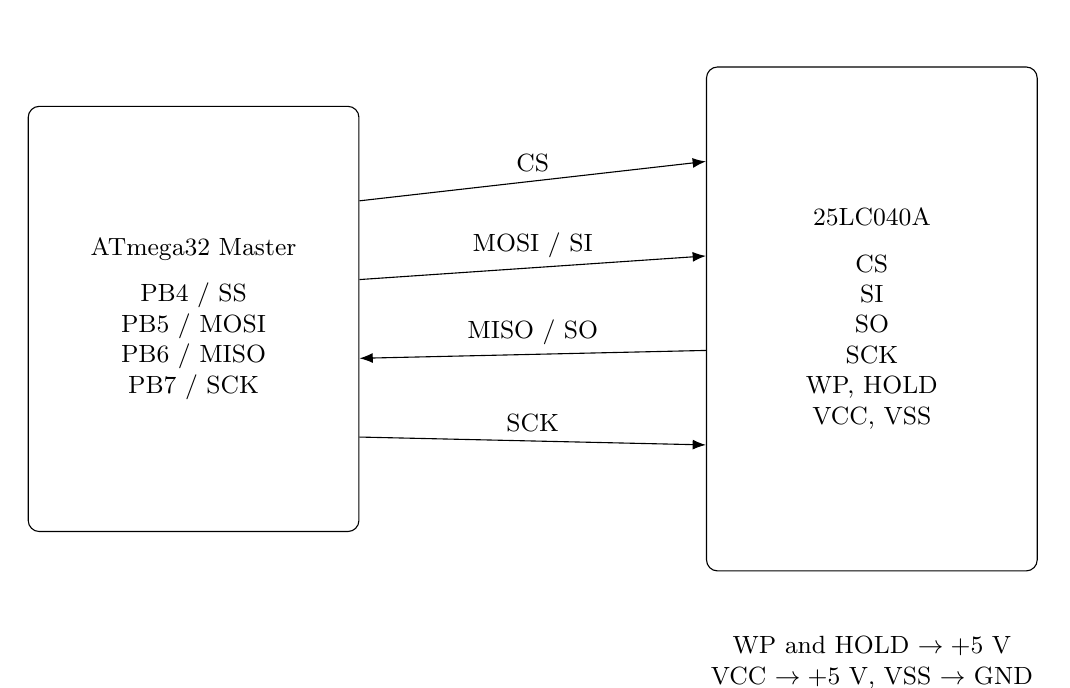
\begin{tikzpicture}[>=Latex, node distance=14mm, every node/.style={font=\small, align=center}]
\node (mcu) [draw, rounded corners, minimum width=42mm, minimum height=54mm, align=center] {ATmega32 Master\\[2mm]
PB4 / SS\\PB5 / MOSI\\PB6 / MISO\\PB7 / SCK};
\node (ee) [draw, rounded corners, right=44mm of mcu, minimum width=42mm, minimum height=64mm, align=center] {25LC040A\\[2mm]
CS\\SI\\SO\\SCK\\WP, HOLD\\VCC, VSS};
\draw[->] ($(mcu.east)+(0,15mm)$) -- node[above]{CS} ($(ee.west)+(0,20mm)$);
\draw[->] ($(mcu.east)+(0,5mm)$) -- node[above]{MOSI / SI} ($(ee.west)+(0,8mm)$);
\draw[<-] ($(mcu.east)+(0,-5mm)$) -- node[above]{MISO / SO} ($(ee.west)+(0,-4mm)$);
\draw[->] ($(mcu.east)+(0,-15mm)$) -- node[above]{SCK} ($(ee.west)+(0,-16mm)$);
\node[below=7mm of ee, align=center] {WP and HOLD $\rightarrow +5$ V\\VCC $\rightarrow +5$ V, VSS $\rightarrow$ GND};
\end{tikzpicture}
\caption{Hardware SPI connection between the Master and 25LC040A.}
\end{figure}

\section{Why Hardware SPI Is Used}
The latest Master implementation uses the ATmega32 hardware SPI peripheral rather than bit-banging the clock and data pins. Hardware SPI provides:
\begin{itemize}
  \item precise clock generation;
  \item automatic serial shifting through \texttt{SPDR};
  \item a completion flag, \texttt{SPIF};
  \item lower CPU overhead and simpler code;
  \item standard use of the dedicated \texttt{PB4--PB7} SPI pins.
\end{itemize}

The Master is the only device that generates the clock. The EEPROM is an SPI slave and responds only while \texttt{CS} is low.

\section{SPI Register Configuration}

\begin{lstlisting}[style=cstyle,caption={SPI EEPROM initialization.}]
void spi_eeprom_init(void)
{
    EE_SPI_DDR |= (1 << EE_SPI_SS) |
                  (1 << EE_SPI_MOSI) |
                  (1 << EE_SPI_SCK);
    EE_SPI_DDR &= ~(1 << EE_SPI_MISO);
    ee_cs_high();

    /* Enable SPI, Master, mode 0, clock F_CPU/16 = 500 kHz @ 8 MHz. */
    SPCR = (1 << SPE) | (1 << MSTR) | (1 << SPR0);
    SPSR = 0x00;
}
\end{lstlisting}

\subsection{Data-direction register}
The Master drives \texttt{SS}, \texttt{MOSI}, and \texttt{SCK}, so they are outputs. The EEPROM drives \texttt{MISO}, so it is an input:
\begin{lstlisting}[style=cstyle]
DDRB4 = 1;  /* CS/SS output */
DDRB5 = 1;  /* MOSI output */
DDRB6 = 0;  /* MISO input  */
DDRB7 = 1;  /* SCK output  */
\end{lstlisting}
Keeping the hardware \texttt{SS} pin configured as an output is also important for preserving SPI Master mode on classic AVR devices.

\subsection{SPCR fields}
The configured value is
\begin{lstlisting}[style=cstyle]
SPCR = (1 << SPE) | (1 << MSTR) | (1 << SPR0);
\end{lstlisting}

\begin{table}[H]
\centering
\caption{SPI Control Register choices.}
\begin{tabular}{clp{0.55\textwidth}}
\toprule
Bit & Field & Selected behavior \\
\midrule
7 & SPIE & Zero: SPI interrupt disabled; transfers are polled. \\
6 & SPE & One: SPI peripheral enabled. \\
5 & DORD & Zero: most-significant bit is transmitted first. \\
4 & MSTR & One: ATmega32 operates as SPI Master. \\
3 & CPOL & Zero: SCK is low while idle. \\
2 & CPHA & Zero: data is sampled on the leading rising edge; SPI mode 0. \\
1:0 & SPR1:SPR0 & \texttt{01}: base clock division of 16 when \texttt{SPI2X=0}. \\
\bottomrule
\end{tabular}
\end{table}

The 25LC040A supports SPI mode 0, so \texttt{CPOL=0} and \texttt{CPHA=0} are appropriate. Mode 0 behavior is:
\begin{itemize}
  \item SCK is low when idle;
  \item output data changes around the falling edge;
  \item input data is sampled on the rising edge.
\end{itemize}

\subsection{SPSR and SPI clock}
The code writes
\begin{lstlisting}[style=cstyle]
SPSR = 0x00;
\end{lstlisting}
so \texttt{SPI2X=0}. With \texttt{SPR1:SPR0=01},
\[
f_{SCK}=\frac{F_{CPU}}{16}=\frac{8\text{ MHz}}{16}=500\text{ kHz}.
\]
A 500 kHz bus is far below the EEPROM maximum and provides generous timing margin in Proteus and real hardware. It is also fast enough that the serial transfer time is negligible compared with the EEPROM's internal write cycle.

\section{Chip-Select Framing}

\begin{lstlisting}[style=cstyle]
static void ee_cs_low(void)
{
    EE_SPI_PORT &= ~(1 << EE_SPI_SS);
}

static void ee_cs_high(void)
{
    EE_SPI_PORT |= (1 << EE_SPI_SS);
}
\end{lstlisting}

\texttt{CS} is active low. A command begins when the Master drives CS low and ends when it returns CS high. The EEPROM interprets bytes according to their position within that interval. CS is set high before enabling SPI so that the EEPROM is not accidentally selected during initialization.

For writes, the low-to-high transition on CS after the command, address, and data have been sent causes the EEPROM to begin its internal self-timed write cycle.

\section{Full-Duplex Byte Transfer}

\begin{lstlisting}[style=cstyle,caption={Hardware SPI byte transfer.}]
static uint8_t spi_transfer(uint8_t data)
{
    SPDR = data;
    while (!(SPSR & (1 << SPIF))) {
        /* wait */
    }
    return SPDR;
}
\end{lstlisting}

SPI is full duplex. For every bit shifted from MOSI, one bit is simultaneously shifted into MISO. Writing a byte to \texttt{SPDR} starts the hardware transfer. The processor polls \texttt{SPIF} until eight clock pulses have completed, then reads the received byte from \texttt{SPDR}.

On the ATmega32, the normal flag-clearing sequence is to read \texttt{SPSR} while \texttt{SPIF} is set and then access \texttt{SPDR}. The polling condition reads \texttt{SPSR}; the return statement reads \texttt{SPDR}, completing that sequence.

At 500 kHz, one bit requires 2 $\mu$s and one byte requires approximately
\[
8\times2\,\mu\text{s}=16\,\mu\text{s}.
\]
Transaction overhead is therefore much shorter than the millisecond-scale internal EEPROM write operation.

\section{25LC040A Instruction Set}

\begin{table}[H]
\centering
\caption{Important 25LC040A instructions.}
\begin{tabular}{clp{0.56\textwidth}}
\toprule
Hex & Mnemonic & Function \\
\midrule
\texttt{0x06} & WREN & Set the write-enable latch before a WRITE or status-register write. \\
\texttt{0x04} & WRDI & Clear the write-enable latch. Supported by the device but not needed by the current driver. \\
\texttt{0x05} & RDSR & Read the status register, including WIP and WEL. \\
\texttt{0x01} & WRSR & Write status-register protection bits. Not used by the project. \\
\texttt{0x03}/\texttt{0x0B} & READ & Read from lower/upper half of memory; bit 3 carries address bit $A_8$. \\
\texttt{0x02}/\texttt{0x0A} & WRITE & Write to lower/upper half of memory; bit 3 carries address bit $A_8$. \\
\bottomrule
\end{tabular}
\end{table}

The project defines the base opcodes:
\begin{lstlisting}[style=cstyle]
#define EE25_WREN   0x06
#define EE25_WRITE  0x02
#define EE25_READ   0x03
#define EE25_RDSR   0x05
\end{lstlisting}
The upper-memory versions are generated by OR-ing bit 3, \texttt{0x08}, into READ or WRITE.

\section{The Ninth Address Bit}

\subsection{Why a ninth bit is necessary}
The memory has 512 byte locations:
\[
512=2^9.
\]
Thus the complete address is
\[
A_8A_7A_6A_5A_4A_3A_2A_1A_0.
\]
Only one address byte follows the instruction, so it can carry $A_7\ldots A_0$. The remaining bit, $A_8$, is encoded in bit 3 of the READ or WRITE instruction.

\subsection{Code implementation}

\begin{lstlisting}[style=cstyle]
spi_transfer((uint8_t)(EE25_WRITE |
             ((addr & 0x0100) ? 0x08 : 0x00)));
spi_transfer((uint8_t)(addr & 0xFF));
\end{lstlisting}

The mask \texttt{0x0100} tests $A_8$. If it is one, \texttt{0x08} is inserted into the command. The following byte contains the lower eight address bits.

\begin{table}[H]
\centering
\caption{Address examples.}
\begin{tabular}{cccccc}
\toprule
Address & $A_8$ & Low byte & READ command & WRITE command & Interpretation \\
\midrule
\texttt{0x07A} & 0 & \texttt{0x7A} & \texttt{0x03} & \texttt{0x02} & Lower half \\
\texttt{0x0FF} & 0 & \texttt{0xFF} & \texttt{0x03} & \texttt{0x02} & Last lower-half byte \\
\texttt{0x100} & 1 & \texttt{0x00} & \texttt{0x0B} & \texttt{0x0A} & First upper-half byte \\
\texttt{0x17A} & 1 & \texttt{0x7A} & \texttt{0x0B} & \texttt{0x0A} & Upper half \\
\texttt{0x1FF} & 1 & \texttt{0xFF} & \texttt{0x0B} & \texttt{0x0A} & Final device byte \\
\bottomrule
\end{tabular}
\end{table}

\begin{figure}[H]
\centering
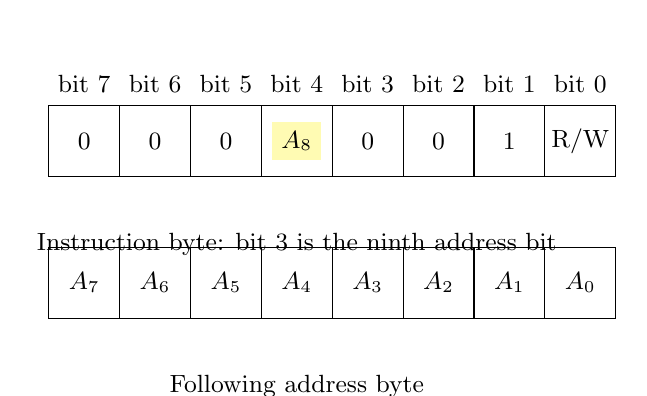
\begin{tikzpicture}[every node/.style={font=\small}, x=9mm, y=9mm]
\foreach \x/\lab in {0/7,1/6,2/5,3/4,4/3,5/2,6/1,7/0} {
  \draw (\x,0) rectangle ++(1,1);
  \node at (\x+0.5,1.3) {bit \lab};
}
\node at (0.5,0.5) {0};
\node at (1.5,0.5) {0};
\node at (2.5,0.5) {0};
\node[fill=yellow!30] at (3.5,0.5) {$A_8$};
\node at (4.5,0.5) {0};
\node at (5.5,0.5) {0};
\node at (6.5,0.5) {1};
\node at (7.5,0.5) {R/W};
\node[below=6mm] at (3.5,0) {Instruction byte: bit 3 is the ninth address bit};

\foreach \x/\lab in {0/A_7,1/A_6,2/A_5,3/A_4,4/A_3,5/A_2,6/A_1,7/A_0} {
  \draw (\x,-2) rectangle ++(1,1);
  \node at (\x+0.5,-1.5) {$\lab$};
}
\node[below=6mm] at (3.5,-2) {Following address byte};
\end{tikzpicture}
\caption{Encoding of the 9-bit address across the command and address bytes. The low opcode bits differ between READ and WRITE.}
\end{figure}

Before every operation, the driver limits the supplied address to the physical range:
\begin{lstlisting}[style=cstyle]
addr &= 0x01FF;
\end{lstlisting}
This keeps only bits $A_8\ldots A_0$ and maps any larger value into the 512-byte address space.

\section{Write-Enable Latch}
EEPROM writes are protected by a write-enable latch, WEL. The Master must issue WREN as a separate CS-framed transaction before each write:

\begin{lstlisting}[style=cstyle]
static void ext_eeprom_write_enable(void)
{
    ee_cs_low();
    spi_transfer(EE25_WREN);
    ee_cs_high();
}
\end{lstlisting}

The separate CS rising edge completes the WREN command and sets WEL. The following WRITE command is then accepted. After the internal write cycle begins or completes, the device automatically clears WEL, so the driver repeats WREN for every byte write.

\section{Writing One Byte}

\begin{lstlisting}[style=cstyle,caption={Single-byte write sequence.}]
void ext_eeprom_write_byte(uint16_t addr, uint8_t data)
{
    addr &= 0x01FF;
    ext_eeprom_write_enable();

    ee_cs_low();
    spi_transfer((uint8_t)(EE25_WRITE |
                 ((addr & 0x0100) ? 0x08 : 0x00)));
    spi_transfer((uint8_t)(addr & 0xFF));
    spi_transfer(data);
    ee_cs_high();

    ext_eeprom_wait_ready();
}
\end{lstlisting}

The complete sequence is:
\begin{enumerate}
  \item Send WREN with its own CS-low interval.
  \item Drive CS low again.
  \item Send WRITE with $A_8$ embedded in bit 3.
  \item Send $A_7\ldots A_0$.
  \item Send the data byte.
  \item Drive CS high, starting the self-timed erase/write cycle.
  \item Poll the WIP status bit until it becomes zero.
\end{enumerate}

\section{Status Register and Ready Polling}

\begin{lstlisting}[style=cstyle,caption={Waiting for the internal write cycle.}]
static void ext_eeprom_wait_ready(void)
{
    uint8_t sr;
    do {
        ee_cs_low();
        spi_transfer(EE25_RDSR);
        sr = spi_transfer(0xFF);
        ee_cs_high();
    } while (sr & 0x01);
}
\end{lstlisting}

The important status bits are:
\begin{table}[H]
\centering
\begin{tabular}{clp{0.57\textwidth}}
\toprule
Bit & Name & Meaning \\
\midrule
0 & WIP & Write in progress. One means the internal write cycle is active. \\
1 & WEL & Write-enable latch. One means a write command is currently permitted. \\
3:2 & BP1:BP0 & Block-protection selection. Left at the device default in this project. \\
7 & WPEN & Status-register hardware write-protect enable. Not configured by this driver. \\
\bottomrule
\end{tabular}
\end{table}

After sending RDSR, the Master sends \texttt{0xFF}. That byte is not meaningful command data; it supplies eight SCK pulses so the EEPROM can shift its status byte onto MISO. Polling rather than using a fixed delay finishes as soon as the device is ready and remains correct across operating conditions.

\section{Reading One Byte}

\begin{lstlisting}[style=cstyle,caption={Single-byte read sequence.}]
uint8_t ext_eeprom_read_byte(uint16_t addr)
{
    uint8_t data;
    addr &= 0x01FF;

    ee_cs_low();
    spi_transfer((uint8_t)(EE25_READ |
                 ((addr & 0x0100) ? 0x08 : 0x00)));
    spi_transfer((uint8_t)(addr & 0xFF));
    data = spi_transfer(0xFF);
    ee_cs_high();

    return data;
}
\end{lstlisting}

The dummy \texttt{0xFF} transfer is required because SPI has no separate ``read'' clock operation. The Master must transmit something to generate the eight clock pulses that shift the selected EEPROM byte onto MISO. The value transmitted during this phase is irrelevant; \texttt{0xFF} is conventional.

\section{Memory Map Used by the Logger}
The logger reserves the first eight bytes as a persistent header and uses the remaining 504 bytes for 63 records:

\begin{table}[H]
\centering
\caption{SmartSafe external EEPROM map.}
\begin{tabular}{lll}
\toprule
Address range & Size & Purpose \\
\midrule
\texttt{0x000--0x007} & 8 bytes & Header: signature, next-write index, valid-record count, reserved bytes \\
\texttt{0x008--0x1FF} & 504 bytes & 63 records $\times$ 8 bytes \\
\bottomrule
\end{tabular}
\end{table}

The constants are:
\begin{lstlisting}[style=cstyle]
#define LOG_HEADER_ADDR  0x000
#define LOG_BASE_ADDR    0x008
#define LOG_RECORD_SIZE  8
#define LOG_MAX_RECORDS  63
#define LOG_MAGIC0       0x53
#define LOG_MAGIC1       0x46
\end{lstlisting}

The two magic bytes are ASCII \texttt{'S'} and \texttt{'F'}. They distinguish a valid initialized SmartSafe log from blank or unrelated EEPROM contents.

\section{Header Format}

\begin{table}[H]
\centering
\caption{Persistent 8-byte header.}
\begin{tabular}{clp{0.55\textwidth}}
\toprule
Offset & Value & Meaning \\
\midrule
0 & \texttt{0x53} & Magic byte 0, ASCII \texttt{S}. \\
1 & \texttt{0x46} & Magic byte 1, ASCII \texttt{F}. \\
2 & \texttt{log\_head} & Index of the next record slot to be written. \\
3 & \texttt{log\_count} & Number of valid records, from 0 through 63. \\
4--7 & \texttt{0xFF} & Reserved for future metadata. \\
\bottomrule
\end{tabular}
\end{table}

\texttt{log\_head} and \texttt{log\_count} are also kept in RAM for fast access. The header is rewritten after every new record so the circular-buffer position survives reset.

\section{Logger Initialization and Clearing}

\begin{lstlisting}[style=cstyle,caption={Persistent-header validation.}]
void logger_init(void)
{
    uint8_t m0 = ext_eeprom_read_byte(LOG_HEADER_ADDR + 0);
    uint8_t m1 = ext_eeprom_read_byte(LOG_HEADER_ADDR + 1);

    if (m0 != LOG_MAGIC0 || m1 != LOG_MAGIC1) {
        log_clear();
        return;
    }

    log_head = ext_eeprom_read_byte(LOG_HEADER_ADDR + 2);
    log_count = ext_eeprom_read_byte(LOG_HEADER_ADDR + 3);

    if (log_head >= LOG_MAX_RECORDS || log_count > LOG_MAX_RECORDS)
        log_clear();
}
\end{lstlisting}

On startup, the logger first checks the signature. Blank EEPROM generally reads as \texttt{0xFF}, so the signature fails and \texttt{log\_clear()} creates a valid empty header. Even when the signature is correct, range checks prevent corrupted metadata from producing out-of-range addresses.

\begin{lstlisting}[style=cstyle]
void log_clear(void)
{
    log_head = 0;
    log_count = 0;
    write_header();
}
\end{lstlisting}

The implementation clears the logical log by resetting metadata. It does not erase every record byte. Old data remains physically present but is no longer included because \texttt{log\_count=0}.

\section{Record Format}
Each event occupies eight bytes:

\begin{table}[H]
\centering
\caption{Event-record structure.}
\begin{tabular}{clp{0.55\textwidth}}
\toprule
Byte & Field & Description \\
\midrule
0 & Event code & One of the \texttt{EVT\_*} constants. \\
1 & Timestamp[31:24] & Most-significant timestamp byte. \\
2 & Timestamp[23:16] & Timestamp byte. \\
3 & Timestamp[15:8] & Timestamp byte. \\
4 & Timestamp[7:0] & Least-significant timestamp byte. \\
5 & Data[15:8] & Optional event-specific data, high byte. \\
6 & Data[7:0] & Optional event-specific data, low byte. \\
7 & Checksum & XOR of bytes 0 through 6. \\
\bottomrule
\end{tabular}
\end{table}

The timestamp is stored big-endian, so the most-significant byte appears first. This produces a consistent byte order independent of the AVR's native little-endian representation.

\section{Checksum}

\begin{lstlisting}[style=cstyle]
static uint8_t checksum7(const uint8_t *b)
{
    uint8_t x = 0;
    for (uint8_t i = 0; i < 7; i++)
        x ^= b[i];
    return x;
}
\end{lstlisting}

The checksum is an XOR of the first seven bytes:
\[
C=b_0\oplus b_1\oplus\cdots\oplus b_6.
\]
It detects many single-bit and simple corruption patterns and is inexpensive on an 8-bit MCU. It is not a cryptographic integrity mechanism and is weaker than a CRC, but it is sufficient for identifying obviously invalid log records in this educational design.

\section{Writing an Event Record}

\begin{lstlisting}[style=cstyle,caption={Record construction and circular-buffer update.}]
void log_event_data(uint8_t event_code,
                    uint32_t timestamp,
                    uint16_t data)
{
    uint8_t r[LOG_RECORD_SIZE];
    uint16_t base;

    if (log_head >= LOG_MAX_RECORDS)
        log_head = 0;

    r[0] = event_code;
    r[1] = (uint8_t)(timestamp >> 24);
    r[2] = (uint8_t)(timestamp >> 16);
    r[3] = (uint8_t)(timestamp >> 8);
    r[4] = (uint8_t)(timestamp);
    r[5] = (uint8_t)(data >> 8);
    r[6] = (uint8_t)(data);
    r[7] = checksum7(r);

    base = LOG_BASE_ADDR +
           (uint16_t)log_head * LOG_RECORD_SIZE;

    for (uint8_t i = 0; i < LOG_RECORD_SIZE; i++)
        ext_eeprom_write_byte(base + i, r[i]);

    log_head++;
    if (log_head >= LOG_MAX_RECORDS)
        log_head = 0;

    if (log_count < LOG_MAX_RECORDS)
        log_count++;

    write_header();
}
\end{lstlisting}

The base address is
\[
base=0x008+8\times log\_head.
\]
After writing, \texttt{log\_head} advances and wraps from 62 back to 0. \texttt{log\_count} increases until it reaches 63, then remains saturated. At that point every new event overwrites the oldest record.

The convenience function
\begin{lstlisting}[style=cstyle]
void log_event(uint8_t event_code, uint32_t timestamp)
{
    log_event_data(event_code, timestamp, 0xFFFF);
}
\end{lstlisting}
uses \texttt{0xFFFF} when an event has no additional 16-bit data.

\section{Circular-Buffer Ordering}
When fewer than 63 records exist, valid records begin at index zero. When the log is full, \texttt{log\_head} points to the oldest record because it is the slot that will be overwritten next. The dump therefore computes:
\begin{lstlisting}[style=cstyle]
uint8_t start = (log_count == LOG_MAX_RECORDS) ? log_head : 0;
\end{lstlisting}
It then walks \texttt{log\_count} records using modulo arithmetic:
\begin{lstlisting}[style=cstyle]
uint8_t idx = (uint8_t)((start + n) % LOG_MAX_RECORDS);
\end{lstlisting}
This prints records from oldest to newest even after several wraparounds.

\section{Log Dump Through USART}
The dump begins and ends with explicit markers:
\begin{lstlisting}[style=cstyle]
usart_print("=== LOG DUMP ===\r\n");
...
usart_print("=== END ===\r\n");
\end{lstlisting}
The Slave uses these markers to ignore log lines while the Virtual Terminal displays them.

For each record, the logger:
\begin{enumerate}
  \item resets the watchdog so a long dump does not reset the Master;
  \item reads all eight bytes;
  \item verifies the checksum;
  \item reconstructs the 32-bit timestamp and 16-bit data field;
  \item prints the index, hexadecimal event code, event name, timestamp, and data.
\end{enumerate}

A typical line is:
\begin{verbatim}
IDX=12 EVT=0x05 POWER_FAIL TS=73s DATA=0xFFFF
\end{verbatim}
A failed checksum is reported as:
\begin{verbatim}
IDX=12 BAD_CHECKSUM
\end{verbatim}

\section{Timing, Performance, and Endurance Considerations}
The current logger intentionally uses the simple byte-write API. One event writes eight record bytes and then eight header bytes. Every byte write requires WREN, a WRITE transaction, and a self-timed write cycle. This is easy to understand and robust for a small academic project, but it is not the most efficient use of the EEPROM.

The device supports page writes, with a page size of 16 bytes. A future optimization could write the complete 8-byte record in one page operation and reduce the header update to fewer cycles. This would shorten event logging and reduce write-cycle consumption. Care must be taken not to cross a page boundary in a single page-write command because data can wrap within the page.

The header is rewritten after every event, so its cells receive more writes than record cells. For a production design, rotating or journaling metadata would improve wear distribution. For the expected event rate of the SmartSafe demonstration, the simple approach is adequate.

\section{Common Hardware and Firmware Faults}

\begin{longtable}{p{0.30\textwidth}p{0.62\textwidth}}
\toprule
Symptom & Likely cause \\
\midrule
\endhead
Driver waits forever in \texttt{ext\_eeprom\_wait\_ready()} & EEPROM unpowered; SO/MISO floating high; SI and SO swapped; HOLD low; incorrect CS wiring. \\
Reads always return \texttt{0xFF} & EEPROM not selected, unpowered, or MISO disconnected; blank memory is also \texttt{0xFF}, so verify SPI waveforms. \\
Writes do not persist & WREN missing; WP/HOLD wiring incorrect; CS not raised between WREN and WRITE; write cycle not completed. \\
Lower half works but upper half fails & Ninth address bit not inserted into command bit 3. \\
SPI exits Master mode unexpectedly & Hardware SS pin configured as an input and driven low; keep PB4 as output. \\
Corrupted records after reset & Header or record write interrupted; checksum identifies incomplete records, but metadata itself currently has no checksum. \\
Terminal dump activates Slave alarm & Slave uses substring matching rather than exact event messages or does not ignore the dump markers. \\
\bottomrule
\end{longtable}

\section{Proteus Verification Procedure}
A systematic test is:
\begin{enumerate}
  \item Confirm CS is high while idle.
  \item Trigger an event and observe a WREN command: CS low, opcode \texttt{0x06}, CS high.
  \item Observe the WRITE command with command, low address byte, and data.
  \item Observe repeated RDSR transactions until WIP clears.
  \item Generate enough events to cross address \texttt{0x0FF}; confirm that upper-half commands become \texttt{0x0A} or \texttt{0x0B}.
  \item Reset the Master and verify that the header restores \texttt{log\_head} and \texttt{log\_count}.
  \item Send the terminal dump command and verify checksum, timestamp, and circular ordering.
\end{enumerate}

Useful logic-analyzer channels are PB4/CS, PB5/MOSI, PB6/MISO, and PB7/SCK.

\section{Complete SPI EEPROM Driver Listing}

\begin{lstlisting}[style=cstyle,caption={Complete hardware-SPI EEPROM driver.}]
/* spi_eeprom.c - Hardware SPI driver for 25LC040 */

#include <avr/io.h>
#include "config.h"
#include "spi_eeprom.h"

static void ee_cs_low(void)
{
    EE_SPI_PORT &= ~(1 << EE_SPI_SS);
}

static void ee_cs_high(void)
{
    EE_SPI_PORT |= (1 << EE_SPI_SS);
}

static uint8_t spi_transfer(uint8_t data)
{
    SPDR = data;
    while (!(SPSR & (1 << SPIF))) {
        /* wait */
    }
    return SPDR;
}

void spi_eeprom_init(void)
{
    EE_SPI_DDR |= (1 << EE_SPI_SS) |
                  (1 << EE_SPI_MOSI) |
                  (1 << EE_SPI_SCK);
    EE_SPI_DDR &= ~(1 << EE_SPI_MISO);
    ee_cs_high();

    SPCR = (1 << SPE) | (1 << MSTR) | (1 << SPR0);
    SPSR = 0x00;
}

static void ext_eeprom_write_enable(void)
{
    ee_cs_low();
    spi_transfer(EE25_WREN);
    ee_cs_high();
}

static void ext_eeprom_wait_ready(void)
{
    uint8_t sr;
    do {
        ee_cs_low();
        spi_transfer(EE25_RDSR);
        sr = spi_transfer(0xFF);
        ee_cs_high();
    } while (sr & 0x01);
}

void ext_eeprom_write_byte(uint16_t addr, uint8_t data)
{
    addr &= 0x01FF;
    ext_eeprom_write_enable();

    ee_cs_low();
    spi_transfer((uint8_t)(EE25_WRITE |
                 ((addr & 0x0100) ? 0x08 : 0x00)));
    spi_transfer((uint8_t)(addr & 0xFF));
    spi_transfer(data);
    ee_cs_high();

    ext_eeprom_wait_ready();
}

uint8_t ext_eeprom_read_byte(uint16_t addr)
{
    uint8_t data;
    addr &= 0x01FF;

    ee_cs_low();
    spi_transfer((uint8_t)(EE25_READ |
                 ((addr & 0x0100) ? 0x08 : 0x00)));
    spi_transfer((uint8_t)(addr & 0xFF));
    data = spi_transfer(0xFF);
    ee_cs_high();

    return data;
}
\end{lstlisting}

\section{Conclusion}
The external EEPROM subsystem combines a conventional ATmega32 hardware-SPI driver with a compact persistent circular log. The most device-specific detail is the ninth address bit: $A_8$ is transmitted in instruction bit 3, producing READ opcodes \texttt{0x03}/\texttt{0x0B} and WRITE opcodes \texttt{0x02}/\texttt{0x0A}. Reliable writes also depend on the separate WREN transaction and WIP polling. Above this driver, the logger uses a validated header, 63 fixed-size records, big-endian timestamps, optional data, and an XOR checksum to preserve and present the SmartSafe event history.

\begin{thebibliography}{9}
\bibitem{eeprom}
Microchip Technology, \emph{25AA040A/25LC040A 4-Kbit SPI Serial EEPROM Data Sheet}.\\
\url{https://ww1.microchip.com/downloads/en/DeviceDoc/21827H.pdf}

\bibitem{atmega32}
Microchip Technology, \emph{ATmega32/L Datasheet}, SPI Serial Peripheral Interface section.\\
\url{https://ww1.microchip.com/downloads/en/DeviceDoc/doc2503.pdf}

\bibitem{project}
SmartSafe Microprocessors End-Term Project Specification, Spring 1404.
\end{thebibliography}

\end{document}
